\chapter{Experimental Results} \label{chap:results}

In this chapter, we begin by describing the experimental setup for the proposed method we present. Then the results of applying the method on several scene configurations are presented. For each configuration we present a comparison between the ideal theoretical results obtained by computing the tensor from given known camera poses, and the practical results obtained from matching image correspondences and estimating the tensor numerically.

\section{Experimental Setup}
The proposed method was implemented in C++, and using the \texttt{ViSP} library. \texttt{ViSP} is an open-source visual servoing framework library developed by \texttt{INRIA} and written in C++ \cite{visp}. It is a modular cross platform library that allows prototyping and developing applications using visual tracking and visual servoing techniques. The implementation is divided into two main classes: Visual Servoing Manager, and Trifocal Tensor.

The Trifocal Tensor class was implemented similar to the available data types classes in \texttt{ViSP}, like Matrices and Vectors. This class is responsible for:
\begin{itemize}
  \item Storing the numerical values of the tensor.
  \item Computing the tensor using pose projection matrices.
  \item Computing the tensor using image correspondences across three images.
  \item Recovering epipoles and projection matrices.
  \item Normalizing the tensor.
  \item Computing the interaction matrix corresponding to the tensor instance.
\end{itemize}

The Visual Servoing Manager class is where the simulator, the scene, and the visual servoing task are defined. The class is responsible for:
\begin{itemize}
  \item Defining the scene configuration, the initial and desired poses.
  \item Storing different instances of the current and desired trifocal tensors.
  \item Computing the control law and velocities of the simulation camera.
  \item Plotting graphs and camera simulations showing the variation of tensor error values, computed velocities, and 3D camera end trajectories.
\end{itemize}

\begin{figure}[ht!]
\centering
\begin{adjustbox}{minipage=.9\linewidth,margin=1ex,bgcolor=black!5,margin=0.3pt,bgcolor=black!30,margin=2ex}
%\begin{mdframed}[linecolor=black!30,backgroundcolor=black!5]
  \centering
  \begin{subfigure}{.48\textwidth}
    \centering
    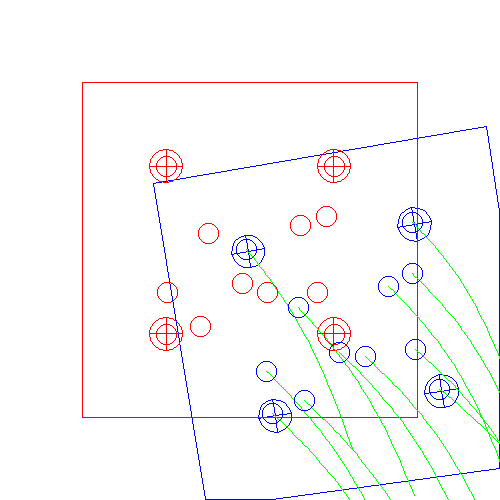
\includegraphics[width=60mm]{figures/rescamera.png}
    \caption{}
    \label{fig:rescamera}
  \end{subfigure}
  \begin{subfigure}{.48\textwidth}
    \centering
    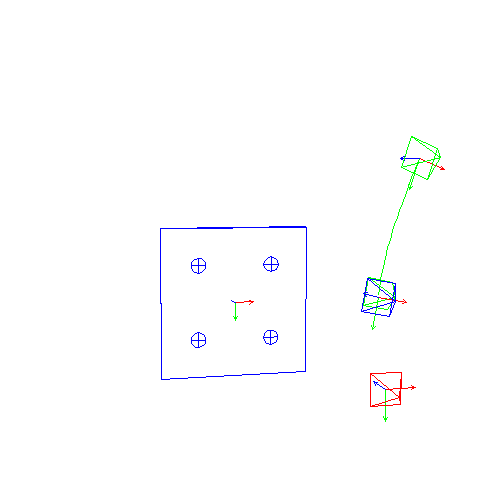
\includegraphics[width=60mm]{figures/resscene.png}
    \caption{}
    \label{fig:resscene}
  \end{subfigure}
  \caption{Experimental Setup (a) Image view with Current/Desired camera projected images plotted in blue/red, with the points trajectory in green. (b) Scene view with initial/current/desired cameras plotted in green/blue/red, with the camera trajectory in green.}
  \label{fig:ressetup}
  %\end{mdframed}
  \end{adjustbox}
\end{figure}

\newpage
The scene setup is defined with two poses for the camera: initial and desired, along with a plate object to be tracked in the scene. A trifocal tensor requires at least 7 non coplanar points for estimating a tensor. Throughout our experiments, we used two sets of 8 and 12 points. There are no much differences between the results of the two sets because we are not considering points mismatch and outliers throughout the experiments. The following results are for the set of 12 points. Throughout the results we show two different views: Image view, and Scene view. Figure \ref{fig:rescamera} shows the image view with projected current and desired camera images plotted in blue and red respectively, along with the points trajectories in green. Figure \ref{fig:resscene} shows the scene view with the position of the initial, current, and desired camera frames plotted in green, blue and red respectively. The resulting camera trajectory is plotted in green.

\section{Experiment I: Pure Translation along x-axis, y-axis}
For first experiment, we consider a pure translational motion along one axis. It's the basic test that can be done to ensure the convergence of the control loop. We consider a small translation of $0.1m$ along x-axis, then y-axis. Figure \ref{fig:ex1p} shows the results of computing the tensor using the pose.  Figure \ref{fig:ex1pvelocity} shows the evolution of the camera velocities, and Figure \ref{fig:ex1perror} shows the evolution of the trifocal tensor coefficients error. Figure \ref{fig:ex1c} shows the results of estimating the tensor through points correspondences. A translation along y-axis produces similar results.

\begin{figure}[ht!]
\begin{mdframed}[linecolor=black!30,backgroundcolor=black!5]
%\begin{adjustbox}{minipage=\linewidth,margin=1ex,bgcolor=black!5,margin=0.3pt,bgcolor=black!30,margin=2ex}
  \centering
  \begin{subfigure}{.48\linewidth}
    \centering
    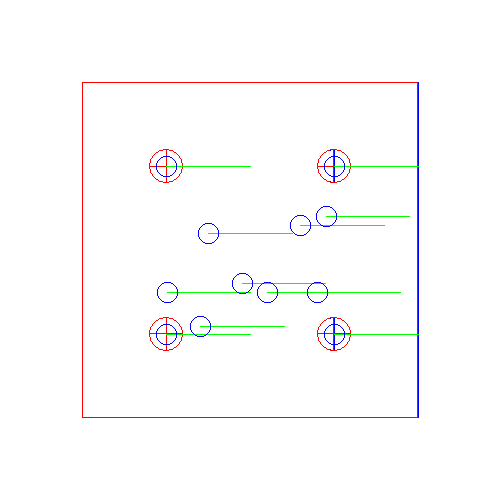
\includegraphics[width=65mm]{figures/plots/ex1pimage.png}
    \caption{}
    \label{fig:ex1pimage}
  \end{subfigure}
  \begin{subfigure}{.48\linewidth}
    \centering
    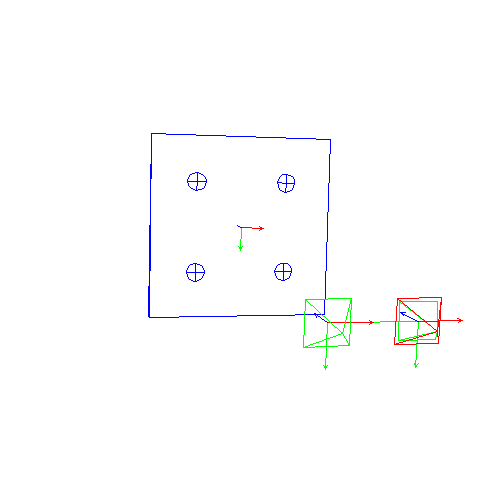
\includegraphics[width=65mm]{figures/plots/ex1pscene.png}
    \caption{}
    \label{fig:ex1pscene}
  \end{subfigure}
  \\
  \begin{subfigure}{.48\linewidth}
    \centering
    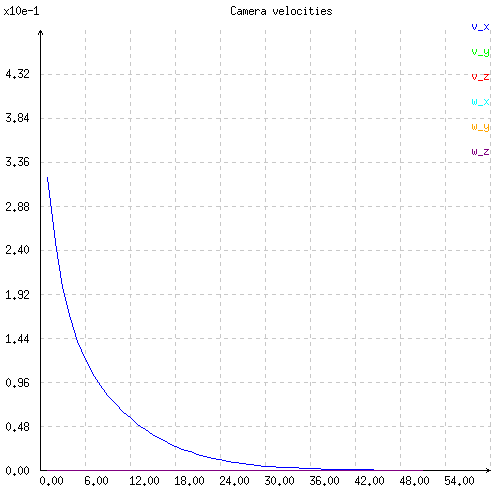
\includegraphics[width=65mm]{figures/plots/ex1pvelocity.png}
    \caption{}
    \label{fig:ex1pvelocity}
  \end{subfigure}
  \begin{subfigure}{.48\linewidth}
    \centering
    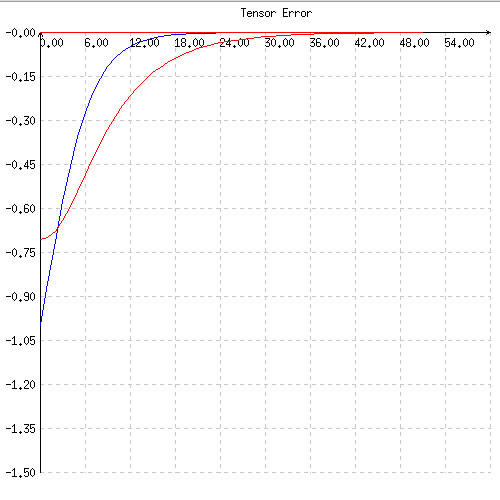
\includegraphics[width=65mm]{figures/plots/ex1perror.png}
    \caption{}
    \label{fig:ex1perror}
  \end{subfigure}
  \caption{Translation along x-axis using tensor from poses. (a) Image view. (b) Scene view. (c) Camera velocities. (d) Tensor coefficients error.}
  \label{fig:ex1p}
\end{mdframed}
%\end{adjustbox}
\end{figure}

\begin{figure}[ht!]
\centering
\begin{mdframed}[linecolor=black!30,backgroundcolor=black!5]
%\begin{adjustbox}{minipage=.8\linewidth,margin=1ex,bgcolor=black!5,margin=0.3pt,bgcolor=black!30,margin=2ex}
  \centering
  \begin{subfigure}{.48\textwidth}
    \centering
    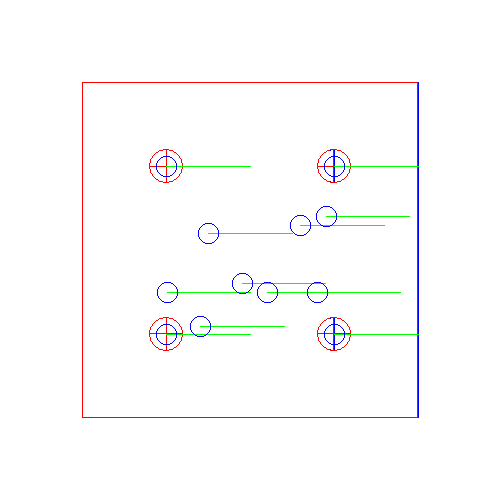
\includegraphics[width=65mm]{figures/plots/ex1pimage.png}
    \caption{}
    \label{fig:ex1cimage}
  \end{subfigure}
  \begin{subfigure}{.48\textwidth}
    \centering
    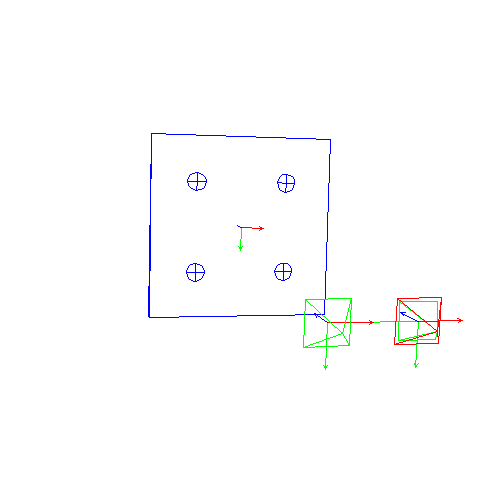
\includegraphics[width=65mm]{figures/plots/ex1pscene.png}
    \caption{}
    \label{fig:ex1cscene}
  \end{subfigure}
  \\
  \begin{subfigure}{.48\textwidth}
    \centering
    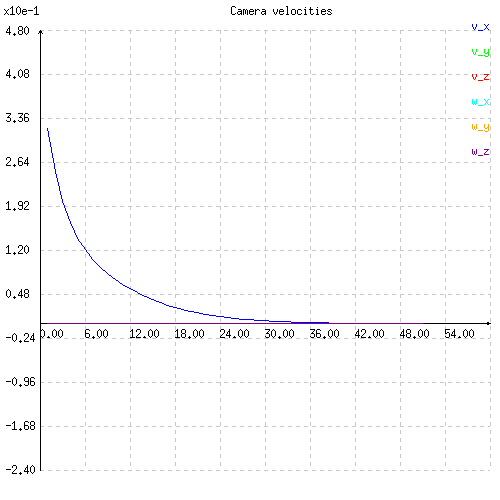
\includegraphics[width=65mm]{figures/plots/ex1cvelocity.png}
    \caption{}
    \label{fig:ex1cvelocity}
  \end{subfigure}
  \begin{subfigure}{.48\textwidth}
    \centering
    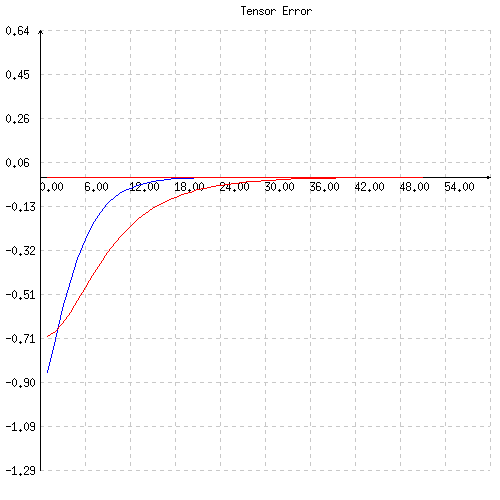
\includegraphics[width=65mm]{figures/plots/ex1cerror.png}
    \caption{}
    \label{fig:ex1cerror}
  \end{subfigure}
  \caption{Translation along x-axis using estimated tensor. (a) Image view. (b) Scene view. (c) Camera velocities. (d) Tensor coefficients error.}
  \label{fig:ex1c}
\end{mdframed}
%\end{adjustbox}
\end{figure}
\clearpage

The system behaviour in both cases is identical. We observe the camera trajectory is linear, which is satisfactory. However, the error is not exactly exponentially decreasing. Several tests were conducted to analyse the source of this behaviour, and it was found that using a subset of tensor coefficients for computing the error and the interaction matrix leads to a perfect exponentially decreasing error. A subset was chosen experimentally to handle this specific configuration, but for different subsets are then required for different configurations. The problem of subset selection is discussed in details in \ref{sec:futurework}. Figure \ref{fig:ex1comparison} shows a comparison between the error plots using all the tensor coefficients and using a subset of them.

\begin{figure}[ht!]
\centering
\begin{adjustbox}{minipage=.9\linewidth,margin=1ex,bgcolor=black!5,margin=0.3pt,bgcolor=black!30,margin=2ex}
  \centering
  \begin{subfigure}{.48\textwidth}
    \centering
    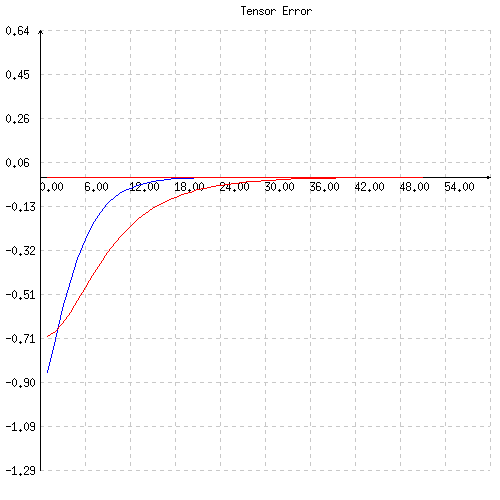
\includegraphics[width=60mm]{figures/plots/ex1cerror.png}
    \caption{}
    \label{fig:ex1comparisona}
  \end{subfigure}
  \begin{subfigure}{.48\textwidth}
    \centering
    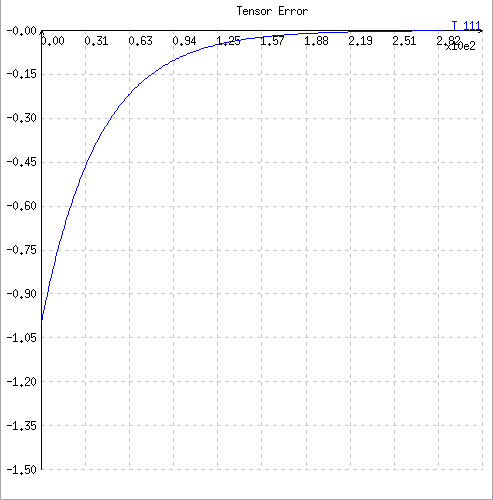
\includegraphics[width=60mm]{figures/plots/ex1subset.png}
    \caption{}
    \label{fig:ex1comparisonb}
  \end{subfigure}
  \caption{Comparison between tensor coefficients error when (a) using all tensor coefficients (b) using a subset of tensor coefficients.}
  \label{fig:ex1comparison}
  \end{adjustbox}
\end{figure}

\section{Experiment II: Pure Translation along z-axis}
Motion along the z-axis is usually more challenging than xyz motion in the IBVS approach. This is due to poor motion resolvability when the camera moves towards the feature points \cite{nelson1996vision}. On the contrary, using the trifocal tensor features this motion is not different than other types of motions. Figure \ref{fig:ex2p} and Figure \ref{fig:ex2c} show the results for the pose and estimated tensors respectively. Like a simple translation along x-axis or y-axis, a translation along z-axis also suffers the problem of selecting a subset of tensor coefficients.

\begin{figure}[ht!]
\begin{mdframed}[linecolor=black!30,backgroundcolor=black!5]
%\begin{adjustbox}{minipage=\linewidth,margin=1ex,bgcolor=black!5,margin=0.3pt,bgcolor=black!30,margin=2ex}
  \centering
  \begin{subfigure}{.48\linewidth}
    \centering
    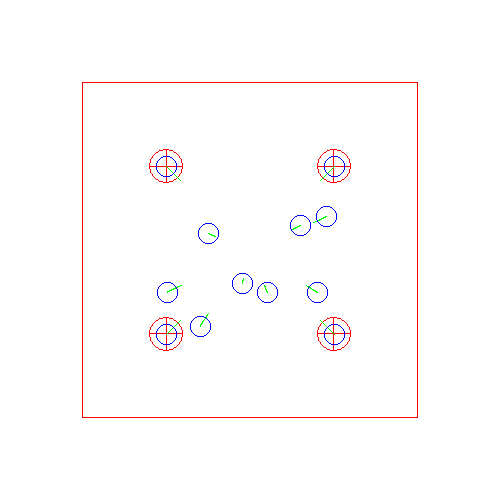
\includegraphics[width=65mm]{figures/plots/ex2pimage.png}
    \caption{}
    \label{fig:ex2pimage}
  \end{subfigure}
  \begin{subfigure}{.48\linewidth}
    \centering
    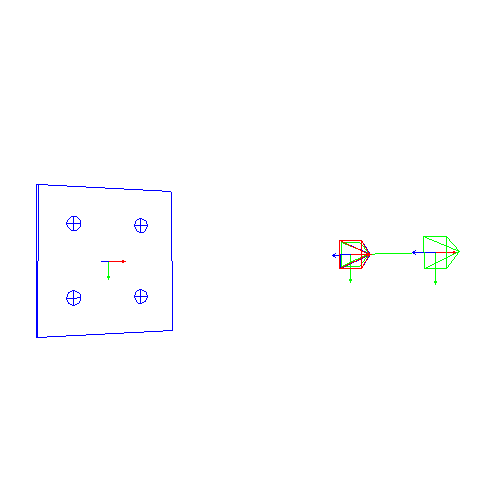
\includegraphics[width=65mm]{figures/plots/ex2pscene.png}
    \caption{}
    \label{fig:ex2pscene}
  \end{subfigure}
  \\
  \begin{subfigure}{.48\linewidth}
    \centering
    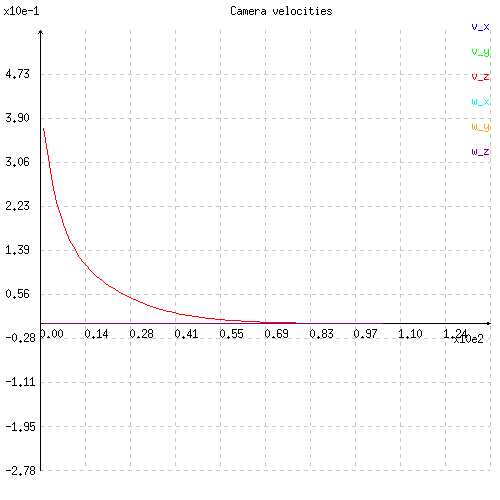
\includegraphics[width=65mm]{figures/plots/ex2pvelocity.png}
    \caption{}
    \label{fig:ex2pvelocity}
  \end{subfigure}
  \begin{subfigure}{.48\linewidth}
    \centering
    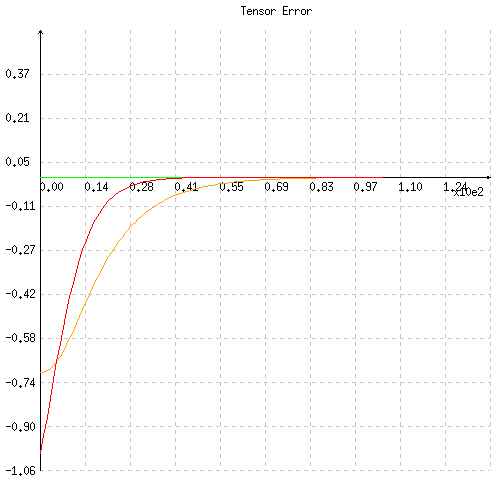
\includegraphics[width=65mm]{figures/plots/ex2perror.png}
    \caption{}
    \label{fig:ex2perror}
  \end{subfigure}
  \caption{Translation along z-axis using tensor from poses. (a) Image view. (b) Scene view. (c) Camera velocities. (d) Tensor coefficients error.}
  \label{fig:ex2p}
\end{mdframed}
%\end{adjustbox}
\end{figure}

\begin{figure}[ht!]
\centering
\begin{mdframed}[linecolor=black!30,backgroundcolor=black!5]
%\begin{adjustbox}{minipage=.8\linewidth,margin=1ex,bgcolor=black!5,margin=0.3pt,bgcolor=black!30,margin=2ex}
  \centering
  \begin{subfigure}{.48\textwidth}
    \centering
    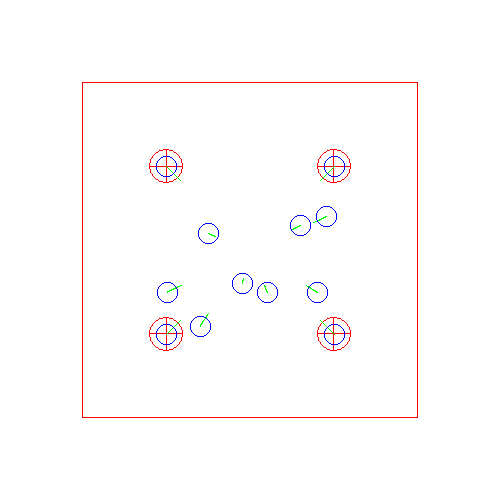
\includegraphics[width=65mm]{figures/plots/ex2pimage.png}
    \caption{}
    \label{fig:ex2cimage}
  \end{subfigure}
  \begin{subfigure}{.48\textwidth}
    \centering
    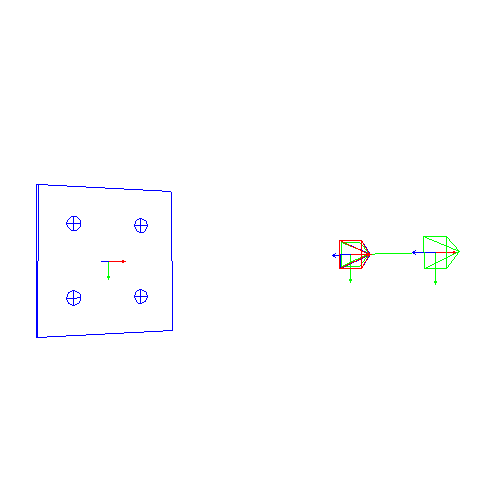
\includegraphics[width=65mm]{figures/plots/ex2pscene.png}
    \caption{}
    \label{fig:ex2cscene}
  \end{subfigure}
  \\
  \begin{subfigure}{.48\textwidth}
    \centering
    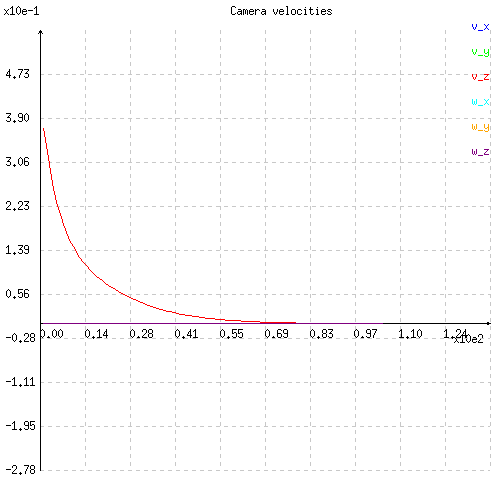
\includegraphics[width=65mm]{figures/plots/ex2cvelocity.png}
    \caption{}
    \label{fig:ex2cvelocity}
  \end{subfigure}
  \begin{subfigure}{.48\textwidth}
    \centering
    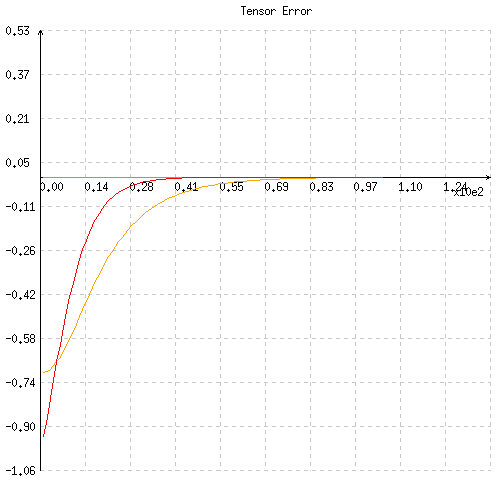
\includegraphics[width=65mm]{figures/plots/ex2cerror.png}
    \caption{}
    \label{fig:ex2cerror}
  \end{subfigure}
  \caption{Translation along z-axis using estimated tensor. (a) Image view. (b) Scene view. (c) Camera velocities. (d) Tensor coefficients error.}
  \label{fig:ex2c}
\end{mdframed}
%\end{adjustbox}
\end{figure}

\section{Experiment III: Translation along xyz-axes}
Now we consider a motion along the 3 x,y, and z axes. From Figure \ref{fig:ex3perror} and \ref{fig:ex3cerror}, we observe the tensor error is not behaving as a desired exponentially decreasing function. However, the camera trajectory is still linear, which is expected and satisfactory.

\begin{figure}[ht!]
\begin{mdframed}[linecolor=black!30,backgroundcolor=black!5]
%\begin{adjustbox}{minipage=\linewidth,margin=1ex,bgcolor=black!5,margin=0.3pt,bgcolor=black!30,margin=2ex}
  \centering
  \begin{subfigure}{.48\linewidth}
    \centering
    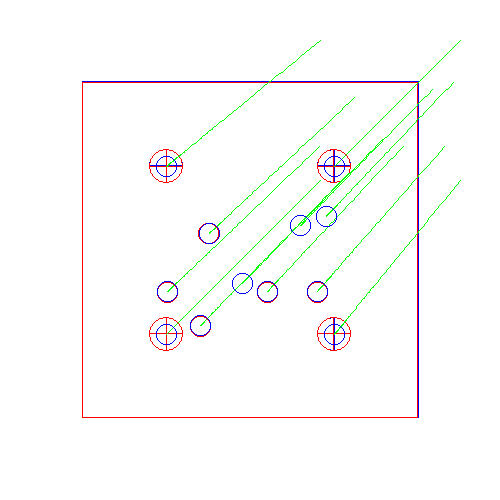
\includegraphics[width=65mm]{figures/plots/ex3pimage.png}
    \caption{}
    \label{fig:ex3pimage}
  \end{subfigure}
  \begin{subfigure}{.48\linewidth}
    \centering
    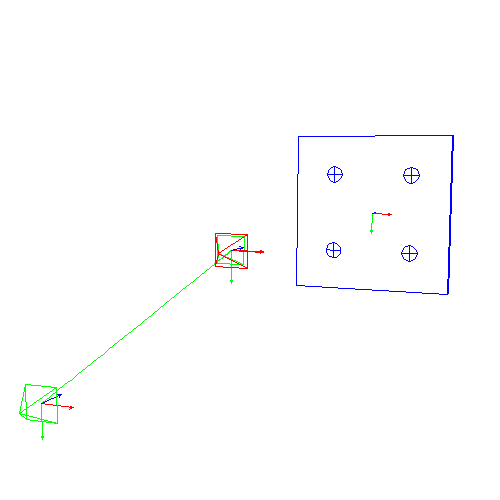
\includegraphics[width=65mm]{figures/plots/ex3pscene.png}
    \caption{}
    \label{fig:ex3pscene}
  \end{subfigure}
  \\
  \begin{subfigure}{.48\linewidth}
    \centering
    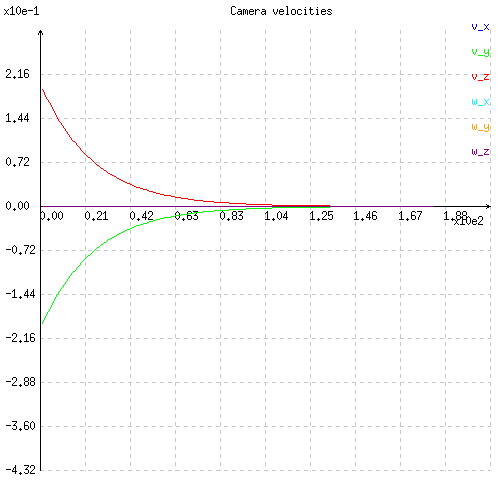
\includegraphics[width=65mm]{figures/plots/ex3pvelocity.png}
    \caption{}
    \label{fig:ex3pvelocity}
  \end{subfigure}
  \begin{subfigure}{.48\linewidth}
    \centering
    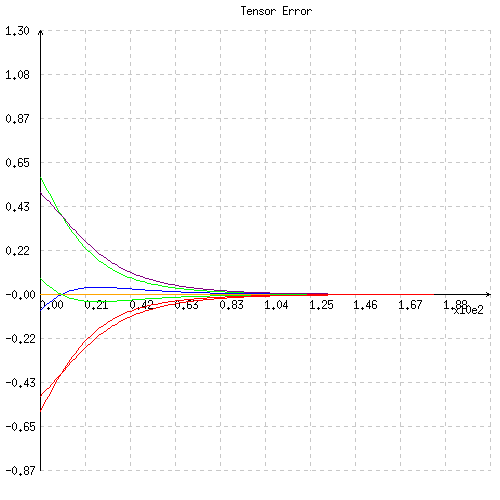
\includegraphics[width=65mm]{figures/plots/ex3perror.png}
    \caption{}
    \label{fig:ex3perror}
  \end{subfigure}
  \caption{Translation along xyz-axes using tensor from poses. (a) Image view. (b) Scene view. (c) Camera velocities. (d) Tensor coefficients error.}
  \label{fig:ex3p}
\end{mdframed}
%\end{adjustbox}
\end{figure}

\begin{figure}[ht!]
\centering
\begin{mdframed}[linecolor=black!30,backgroundcolor=black!5]
%\begin{adjustbox}{minipage=.8\linewidth,margin=1ex,bgcolor=black!5,margin=0.3pt,bgcolor=black!30,margin=2ex}
  \centering
  \begin{subfigure}{.48\textwidth}
    \centering
    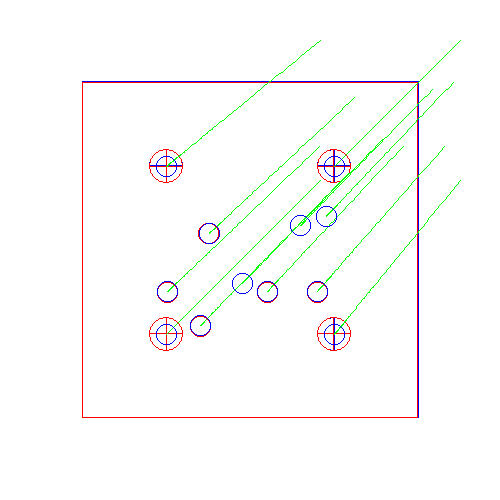
\includegraphics[width=65mm]{figures/plots/ex3cimage.png}
    \caption{}
    \label{fig:ex3cimage}
  \end{subfigure}
  \begin{subfigure}{.48\textwidth}
    \centering
    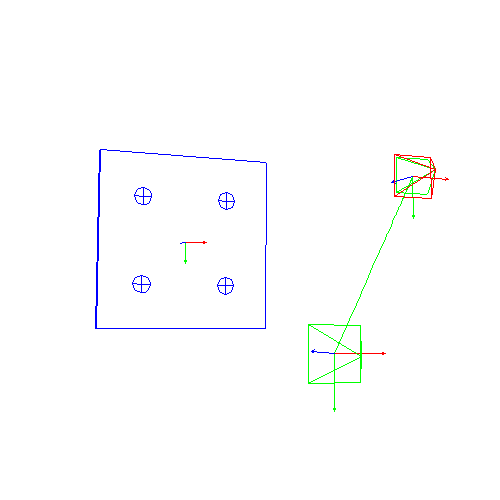
\includegraphics[width=65mm]{figures/plots/ex3cscene.png}
    \caption{}
    \label{fig:ex3cscene}
  \end{subfigure}
  \\
  \begin{subfigure}{.48\textwidth}
    \centering
    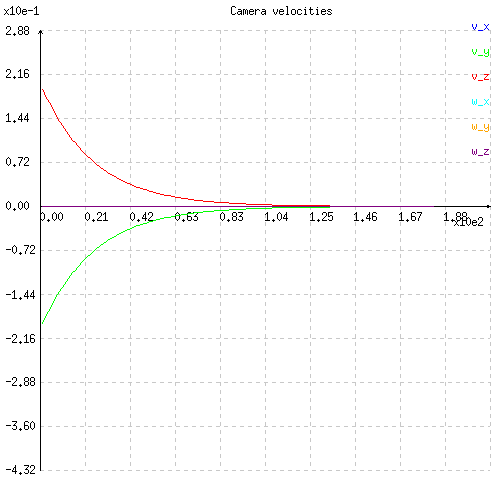
\includegraphics[width=65mm]{figures/plots/ex3cvelocity.png}
    \caption{}
    \label{fig:ex3cvelocity}
  \end{subfigure}
  \begin{subfigure}{.48\textwidth}
    \centering
    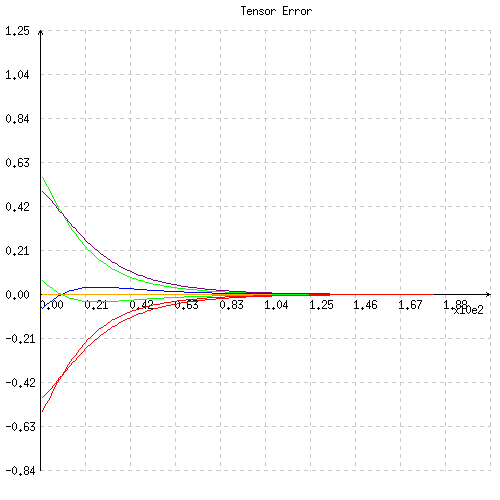
\includegraphics[width=65mm]{figures/plots/ex3cerror.png}
    \caption{}
    \label{fig:ex3cerror}
  \end{subfigure}
  \caption{Translation along xyz-axes using estimated tensor. (a) Image view. (b) Scene view. (c) Camera velocities. (d) Tensor coefficients error.}
  \label{fig:ex3c}
\end{mdframed}
%\end{adjustbox}
\end{figure}

\section{Experiment IV: Large rotation around z-axis}
One of the most challenging IBVS configurations is the $180$\textdegree rotation around the z-axis \cite{chaumette2006visual}\cite{chaumette1998potential}. This is due to the nature of the image-based control law which makes the camera retreat from the object instead of rotating around the z-axis. It is important to evaluate the visual servoing method for large z-axis rotations, close to $180$\textdegree.

Here we consider a translation of $1m$ and a $170$\textdegree rotation. As we can observe in Figure \ref{fig:ex4p} and Figure \ref{fig:ex4c}, the retreat problem didn't occur. The image trajectories follow a spiral motion, which is exactly as expected due to the linear motion for the translation, and the rotational motion for the rotation.

\begin{figure}[ht!]
\begin{mdframed}[linecolor=black!30,backgroundcolor=black!5]
%\begin{adjustbox}{minipage=\linewidth,margin=1ex,bgcolor=black!5,margin=0.3pt,bgcolor=black!30,margin=2ex}
  \centering
  \begin{subfigure}{.48\linewidth}
    \centering
    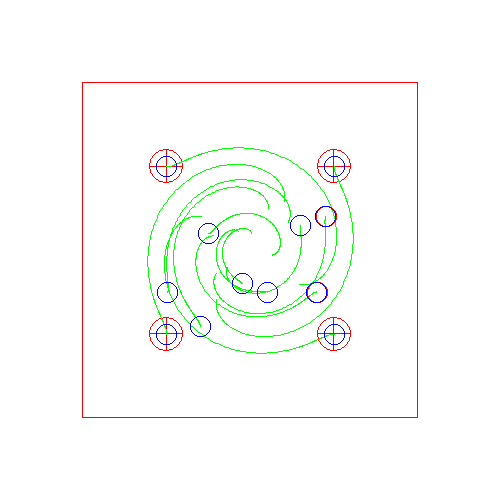
\includegraphics[width=65mm]{figures/plots/ex4pimage.png}
    \caption{}
    \label{fig:ex4pimage}
  \end{subfigure}
  \begin{subfigure}{.48\linewidth}
    \centering
    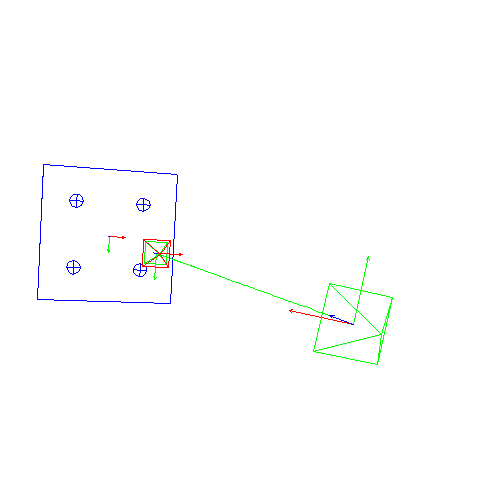
\includegraphics[width=65mm]{figures/plots/ex4pscene.png}
    \caption{}
    \label{fig:ex4pscene}
  \end{subfigure}
  \\
  \begin{subfigure}{.48\linewidth}
    \centering
    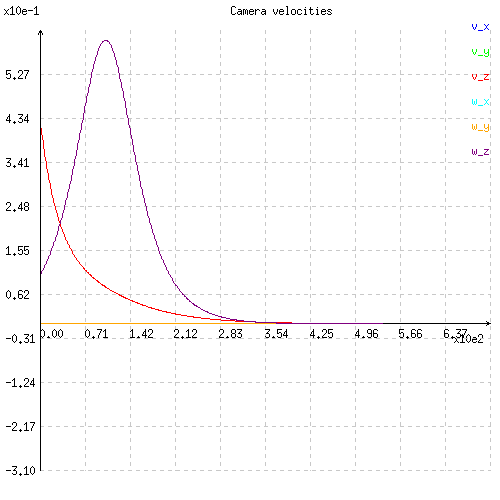
\includegraphics[width=65mm]{figures/plots/ex4pvelocity.png}
    \caption{}
    \label{fig:ex4pvelocity}
  \end{subfigure}
  \begin{subfigure}{.48\linewidth}
    \centering
    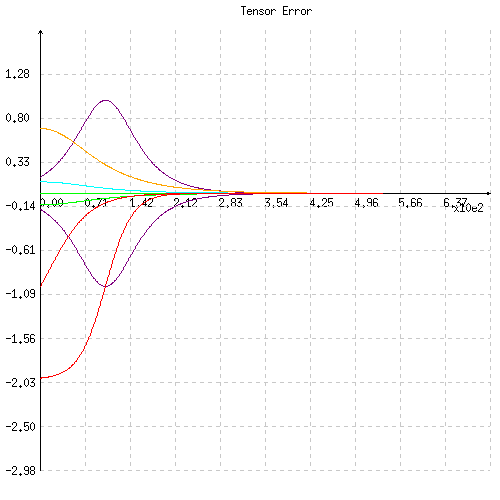
\includegraphics[width=65mm]{figures/plots/ex4perror.png}
    \caption{}
    \label{fig:ex4perror}
  \end{subfigure}
  \caption{Translation and large rotation along z-axis using tensor from poses. (a) Image view. (b) Scene view. (c) Camera velocities. (d) Tensor coefficients error.}
  \label{fig:ex4p}
\end{mdframed}
%\end{adjustbox}
\end{figure}

\begin{figure}[ht!]
\centering
\begin{mdframed}[linecolor=black!30,backgroundcolor=black!5]
%\begin{adjustbox}{minipage=.8\linewidth,margin=1ex,bgcolor=black!5,margin=0.3pt,bgcolor=black!30,margin=2ex}
  \centering
  \begin{subfigure}{.48\textwidth}
    \centering
    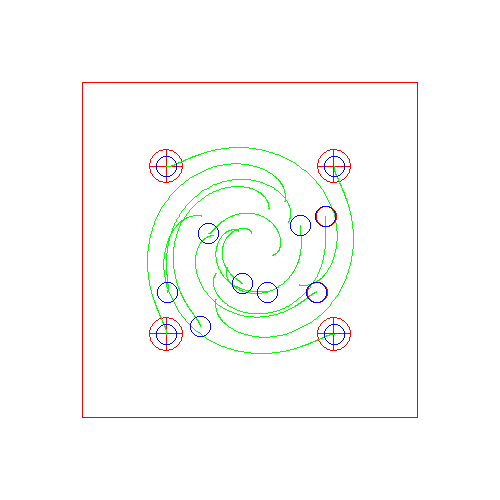
\includegraphics[width=65mm]{figures/plots/ex4cimage.png}
    \caption{}
    \label{fig:ex4cimage}
  \end{subfigure}
  \begin{subfigure}{.48\textwidth}
    \centering
    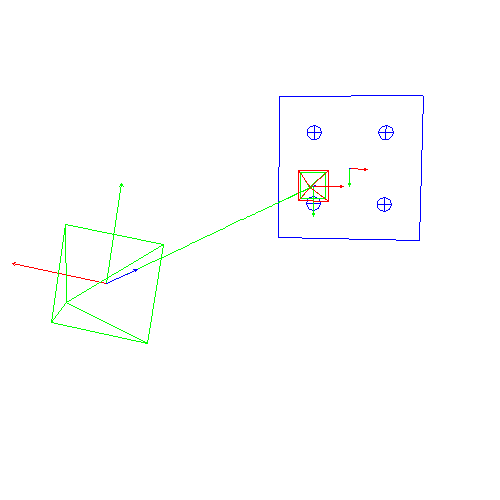
\includegraphics[width=65mm]{figures/plots/ex4cscene.png}
    \caption{}
    \label{fig:ex4cscene}
  \end{subfigure}
  \\
  \begin{subfigure}{.48\textwidth}
    \centering
    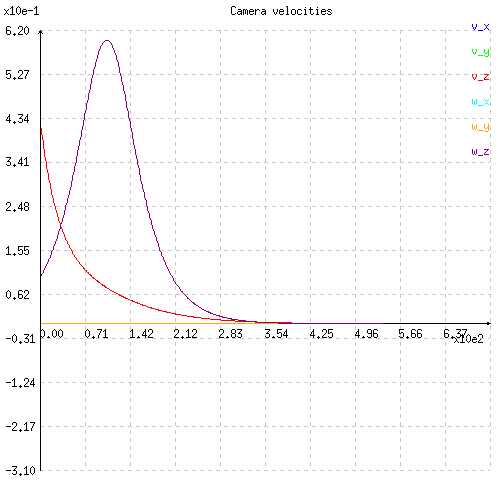
\includegraphics[width=65mm]{figures/plots/ex4cvelocity.png}
    \caption{}
    \label{fig:ex4cvelocity}
  \end{subfigure}
  \begin{subfigure}{.48\textwidth}
    \centering
    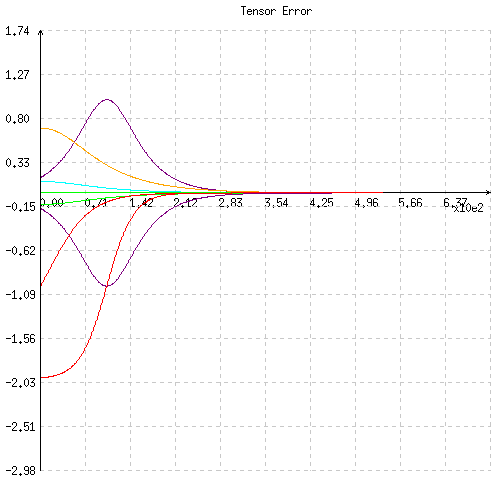
\includegraphics[width=65mm]{figures/plots/ex4cerror.png}
    \caption{}
    \label{fig:ex4cerror}
  \end{subfigure}
  \caption{Translation and large rotation along z-axis using estimated tensor. (a) Image view. (b) Scene view. (c) Camera velocities. (d) Tensor coefficients error.}
  \label{fig:ex4c}
\end{mdframed}
%\end{adjustbox}
\end{figure}

\section{Experiment V: Generic Motion}
In this experiment, we choose a generic camera motion: translations of $0.25m, -0.3m, 0.2m$, and rotations of $10\text{\textdegree}, -20\text{\textdegree}, 5\text{\textdegree}$ along x,y, and z axes respectively. The results in Figures \ref{fig:ex5p} and \ref{fig:ex5c} show smooth camera and image trajectories. However, comparing the two Figures \ref{fig:ex5pvelocity} and \ref{fig:ex5cvelocity}, we notice small oscillations in the camera velocities initially. Lopez-Nicolas \cite{lopez2010visual} mentioned similar oscillations due to noise during image points extraction and matching. Although in our case we omit points mismatch and outliers, but this behaviour is most likely due to small numerical error in the trifocal tensor estimation, as the pose tensor doesn't produce similar oscillations.

\begin{figure}[ht!]
\begin{mdframed}[linecolor=black!30,backgroundcolor=black!5]
%\begin{adjustbox}{minipage=\linewidth,margin=1ex,bgcolor=black!5,margin=0.3pt,bgcolor=black!30,margin=2ex}
  \centering
  \begin{subfigure}{.48\linewidth}
    \centering
    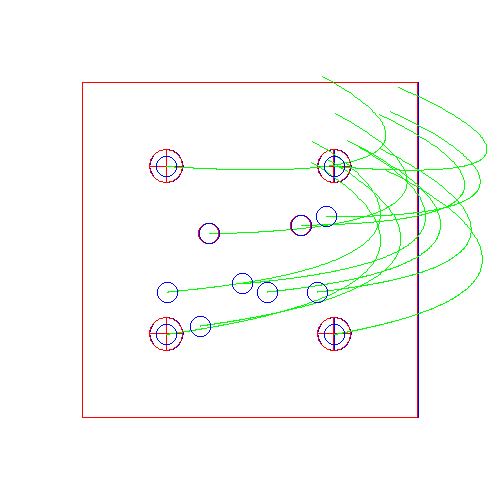
\includegraphics[width=65mm]{figures/plots/ex5pimage.png}
    \caption{}
    \label{fig:ex5pimage}
  \end{subfigure}
  \begin{subfigure}{.48\linewidth}
    \centering
    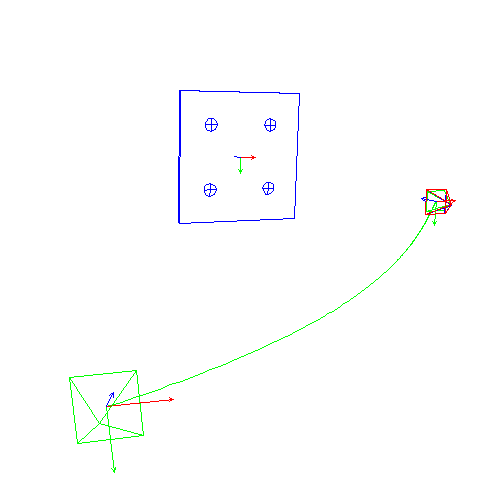
\includegraphics[width=65mm]{figures/plots/ex5pscene.png}
    \caption{}
    \label{fig:ex5pscene}
  \end{subfigure}
  \\
  \begin{subfigure}{.48\linewidth}
    \centering
    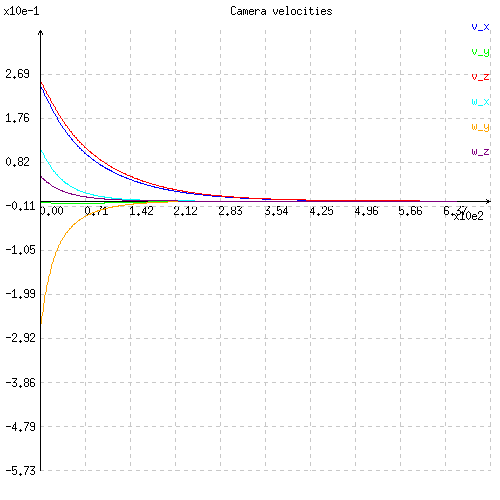
\includegraphics[width=65mm]{figures/plots/ex5pvelocity.png}
    \caption{}
    \label{fig:ex5pvelocity}
  \end{subfigure}
  \begin{subfigure}{.48\linewidth}
    \centering
    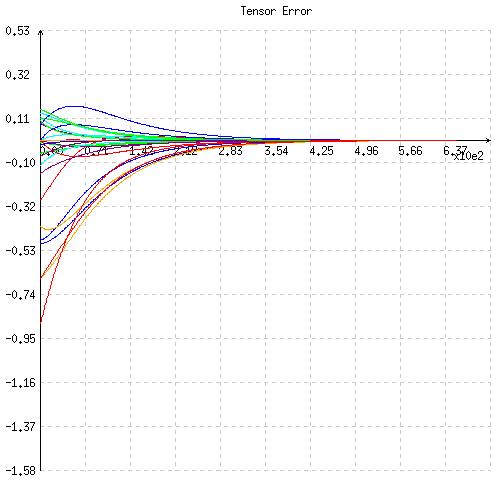
\includegraphics[width=65mm]{figures/plots/ex5perror.png}
    \caption{}
    \label{fig:ex5perror}
  \end{subfigure}
  \caption{Generic motion using tensor from poses. (a) Image view. (b) Scene view. (c) Camera velocities. (d) Tensor coefficients error.}
  \label{fig:ex5p}
\end{mdframed}
%\end{adjustbox}
\end{figure}

\begin{figure}[ht!]
\centering
\begin{mdframed}[linecolor=black!30,backgroundcolor=black!5]
%\begin{adjustbox}{minipage=.8\linewidth,margin=1ex,bgcolor=black!5,margin=0.3pt,bgcolor=black!30,margin=2ex}
  \centering
  \begin{subfigure}{.48\textwidth}
    \centering
    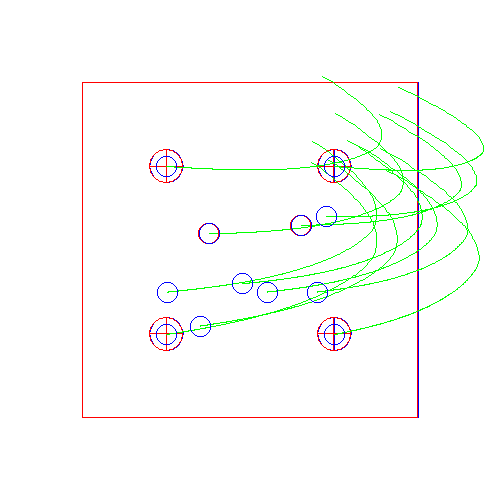
\includegraphics[width=65mm]{figures/plots/ex5cimage.png}
    \caption{}
    \label{fig:ex5cimage}
  \end{subfigure}
  \begin{subfigure}{.48\textwidth}
    \centering
    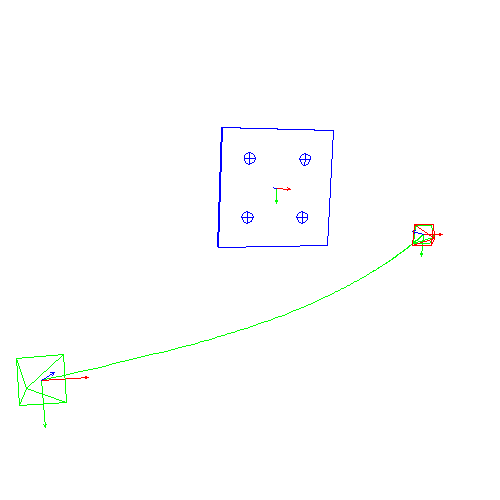
\includegraphics[width=65mm]{figures/plots/ex5cscene.png}
    \caption{}
    \label{fig:ex5cscene}
  \end{subfigure}
  \\
  \begin{subfigure}{.48\textwidth}
    \centering
    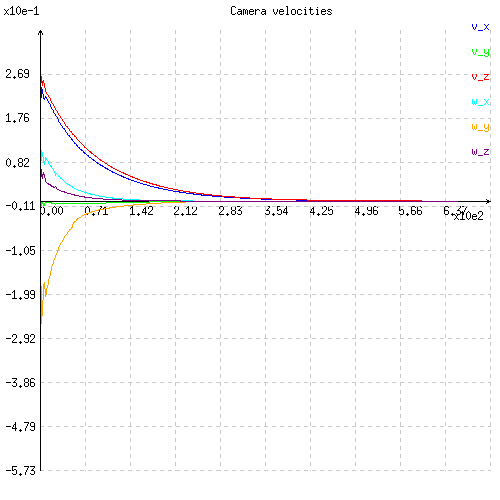
\includegraphics[width=65mm]{figures/plots/ex5cvelocity.png}
    \caption{}
    \label{fig:ex5cvelocity}
  \end{subfigure}
  \begin{subfigure}{.48\textwidth}
    \centering
    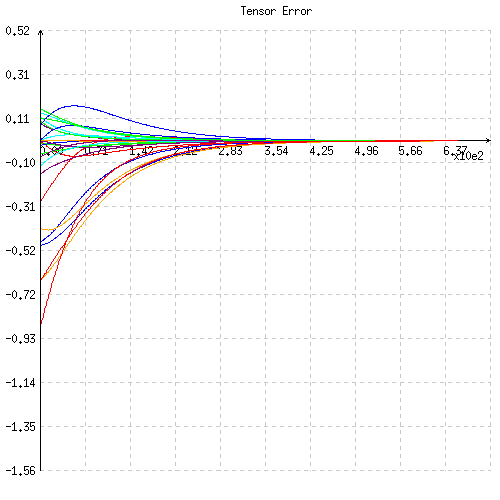
\includegraphics[width=65mm]{figures/plots/ex5cerror.png}
    \caption{}
    \label{fig:ex5cerror}
  \end{subfigure}
  \caption{Generic motion using estimated tensor. (a) Image view. (b) Scene view. (c) Camera velocities. (d) Tensor coefficients error.}
  \label{fig:ex5c}
\end{mdframed}
%\end{adjustbox}
\end{figure}
